\section{Исследование системы массового обслуживания}
\label{sec:part1}

\subsection{Структура и проверка по УИР 2}

Исследуемая система состоит из двух параллельных ветвей.
В ветвь П1 направляется \(75\%\) заявок, в П2 — \(25\%\).
Перед П1 предусмотрено два места ожидания, перед П2 — одно.
При заполнении выбранной ветви заявка теряется. Среднее время
экспоненциального обслуживания в каждой ветви составляет \(5\) с.
Начальная контрольная точка соответствует интенсивности
\(\lambda=0{,}6\) заявки/с, принятой для системы 33 в УИР~2.

Суммарную ёмкость ветви в GPSS задаёт \texttt{STORAGE Cap},
ёмкость обслуживания — \texttt{STORAGE Srv}. Перед входом
\texttt{TEST} проверяет свободное место, блоки \texttt{QUEUE}
и \texttt{DEPART} регистрируют ожидание, а задержка в \texttt{ADVANCE}
соответствует обслуживанию. Заявка завершает обслуживание в
\texttt{Done}, отказ регистрируется в \texttt{Lost}.
Для расчёта \(\overline W\) и \(\overline T\) используются заявки,
закончившие обслуживание. Доля потерь определяется среди всех
завершившихся исходов, включая отказы. Значения по отдельным
приборам суммируются для загрузки и длины очереди.

\begin{table}[htbp]
  \centering
  \caption{Сверка исходной точки системы 33}
  \label{tab:p1-baseline}
  \begin{tabular}{@{}lrrr@{}}
  \toprule
  Характеристика & УИР~2 & GPSS World & Отклонение, \% \\
  \midrule
  Среднее число занятых приборов & 1,516814 & 1,518697 & $+0,12$\\
  Производительность, заявок/с & 0,303363 & 0,304447 & $+0,36$\\
  Вероятность потери & 0,494395 & 0,491417 & $-0,60$\\
  Средняя суммарная длина очереди & 1,656407 & 1,649222 & $-0,43$\\
  Среднее время ожидания, с & 5,460153 & 5,416749 & $-0,79$\\
  Среднее время пребывания, с & 10,460153 & 10,405015 & $-0,53$\\
  \bottomrule
  \end{tabular}
\end{table}

В измерительном интервале длиной \(200\,462{,}1\) с получено
\(61\,030\) завершений обслуживания и \(58\,970\) отказов.
Стандартный отчёт этого прогона показан на
рисунке~\ref{fig:gp-system-report}.
Наибольшее относительное отклонение в таблице~\ref{tab:p1-baseline}
составило \(0{,}79\%\). По формуле Литтла \(X\overline W=1{,}6491\),
что согласуется с интегральным средним числа заявок в очередях.
Отклонение от стационарного расчёта ожидаемо при конечной
длительности прогона.

\subsection{Эксперименты с потоком и обслуживанием}

Предложенная загрузка одного прибора в первой ветви задаётся как
\(\rho_1=0{,}75b/a\), где \(a\) — средний интервал на входе,
\(b\) — средняя длительность обслуживания, а \(0{,}75\) — вероятность
выбора ветви. Средний интервал \(a=11{,}5167\) с сохранён для всех
четырёх потоков. Значения \(\rho_1=0{,}50;\,0{,}75;\,0{,}95;\,0{,}99\)
получены подбором \(b\).

В GPSS World сравнивались простейший поток, циклическая трасса из
300 интервалов варианта 207, равномерный поток с интервалами из
\([0;2a]\) и гиперэкспоненциальная аппроксимация \(H_2\) из УИР~1.
Программа УИР~1 читала первую колонку исходного файла, содержащую
целые части интервалов. Для согласованности здесь повторно использована
эта последовательность со средним \(11{,}5167\) с и коэффициентом
вариации \(2{,}429\). Нулевые интервалы порождают заявки с одинаковым
временем поступления. Вес длинной фазы аппроксимации равен \(0{,}2319\).
Средние фаз \(44{,}32\) и \(1{,}61\) с масштабированы общим множителем,
чтобы среднее смеси совпало со средним трассы.

Параметрические серии выполнены средствами GPSS World. Для каждого
основного режима проведено три повтора по \(120\,000\) исходов после
\(10\,000\) исходов прогрева. В дополнительной серии изменения
\(a\) и \(b\) при простейшем потоке использован один прогон на режим.
Перед измерением команда \texttt{RESET}
сбрасывает статистику. Процедура PLUS записывает из модели значения
системных атрибутов и счётчики по завершении каждого прогона. В
таблицах приведены средние по повторам и суммарное число отказов.
Полосы на графиках показывают \(95\%\)-е интервалы Стьюдента по средним
отдельных повторов. Для трассы интервалы отражают разброс результатов
при разных реализациях маршрутизации и обслуживания на фиксированном
входе.

\begin{figure}[htbp]
 \centering
 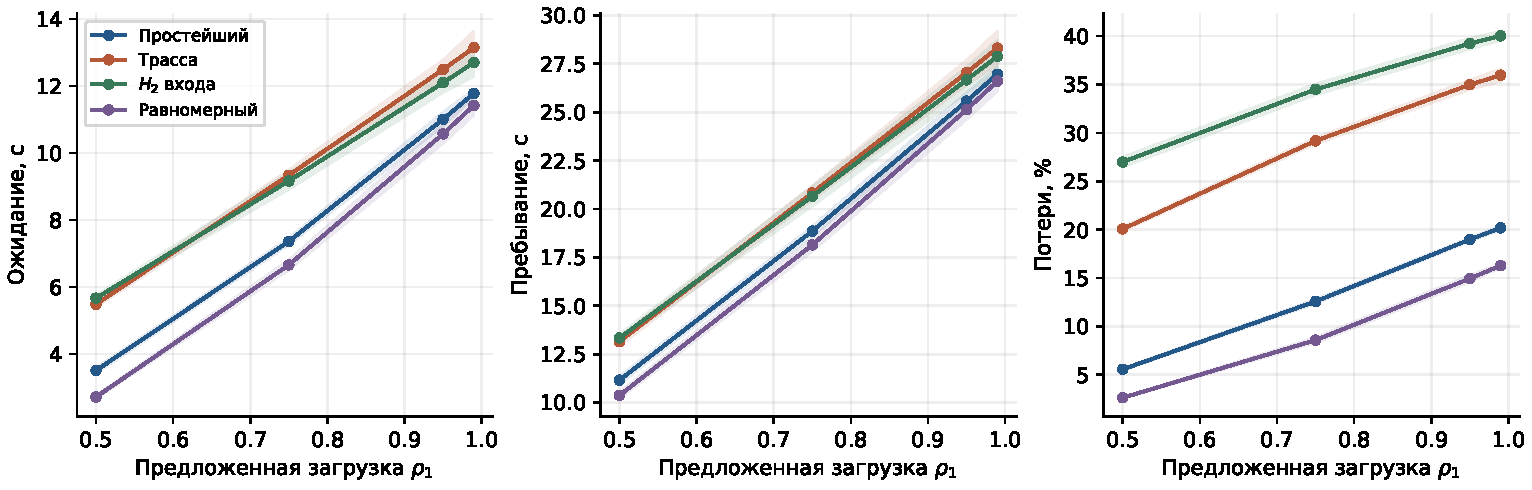
\includegraphics[width=\textwidth]{../out/part1/gpss/flows.pdf}
 \caption{Ожидание, пребывание и потери при смене входного потока}
 \label{fig:p1-flows}
\end{figure}

При простейшем потоке сравнивались экспоненциальный, эрланговский и
гиперэкспоненциальный законы обслуживания обоих приборов. Для \(E_2\)
длительность равна сумме двух экспоненциальных фаз со средним \(b/2\).
Для \(H_2\) с коэффициентом вариации 2 использованы веса
\(p=(1+\sqrt{3/5})/2\), \(1-p\) и средние фаз \(b/(2p)\),
\(b/[2(1-p)]\). Среднее обслуживания во всех случаях равно \(b\).

\begin{table}[htbp]
 \centering\small
 \caption{Смена входного потока или обслуживания при \(\rho_1=0{,}75\)}
 \label{tab:p1-flow-service}
 \begin{tabular}{@{}lrrrrrrr@{}}
 \toprule
 Вариант & Занято & Отказов & Потери, \% &
 \(\overline W\), с & \(\sigma_W\), с & \(\overline T\), с & \(\sigma_T\), с\\
 \midrule
 \TableRows ../out/part1/gpss/flow_service_rows.tex
 \bottomrule
 \end{tabular}
\end{table}

В первых четырёх строках таблицы~\ref{tab:p1-flow-service} фиксирован
экспоненциальный закон обслуживания. Последние две строки сравниваются
с первой при одинаковом простейшем потоке. Среднеквадратические
отклонения определены по заявкам, завершившим обслуживание.
Показатель «Занято» — среднее число занятых приборов в двух ветвях.
При замене входного потока доля потерь выросла с \(12{,}57\%\) до
\(29{,}17\%\) для трассы и до \(34{,}48\%\) для \(H_2\).
Короткие интервалы в этих потоках приводят к поступлению заявок
группами, и накопители быстрее заполняются. Равномерный поток
дал \(8{,}58\%\) потерь. При изменении обслуживания доля потерь
составила \(10{,}30\%\) для \(E_2\) и \(18{,}27\%\) для \(H_2\).
При \(\rho_1=0{,}99\) среднее ожидание простейшего режима равно
\(11{,}78\) с. Замена входа на \(H_2\) увеличила его до \(12{,}70\) с,
а замена обслуживания на \(H_2\) — до \(13{,}72\) с.

\begin{figure}[htbp]
 \centering
 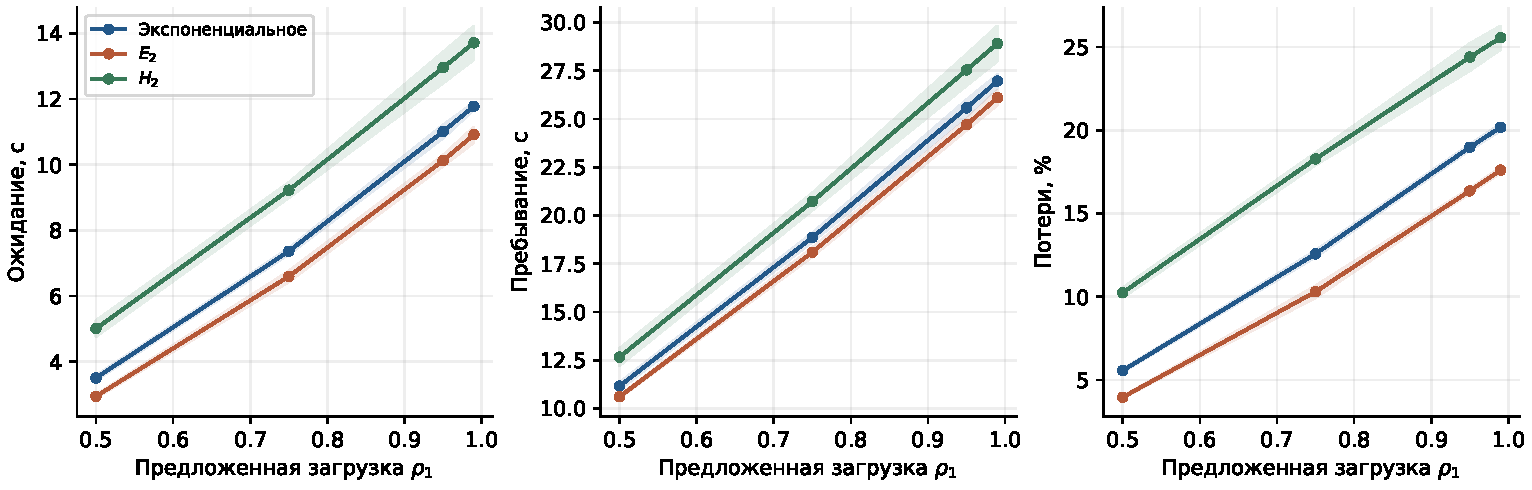
\includegraphics[width=\textwidth]{../out/part1/gpss/services.pdf}
 \caption{Характеристики СМО при смене закона обслуживания}
 \label{fig:p1-services}
\end{figure}

\subsection{Переходный режим}

Модель запускалась из пустого состояния. Накопленные оценки
\(\overline W\) и доли потерь после \(10\), \(50\), \(100\), \(200\),
\(300\), \(600\), \(1200\), \(2500\), \(5000\) и \(10\,000\) исходов
сравнивались со средними после прогрева. Точкой стабилизации принят
первый контрольный момент, начиная с которого все оставшиеся точки,
числом не меньше двух, укладываются в допуск. Для доли потерь допуск
составляет \(0{,}005\) по абсолютной величине, для ожидания — \(5\%\)
с нижней границей \(0{,}02\) с. В таблицах прочерк означает, что
на проверенной сетке критерий не выполнен. Выбор контрольных моментов
и начальное состояние влияют на полученную оценку.

\begin{table}[htbp]
 \centering\small
 \caption{Число исходов до стабилизации оценок для разных потоков}
 \label{tab:p1-transition}
 \begin{tabular}{@{}rrrr@{}}
 \toprule
 \(\rho_1\) & Простейший & Трасса & Аппроксимация \(H_2\)\\
 \midrule
 \TableRows ../out/part1/gpss/transition_rows.tex
 \bottomrule
 \end{tabular}
\end{table}

При простейшем потоке и \(\rho_1=0{,}75\) обе оценки вошли в допуск
с \(5000\) исходов. На той же загрузке трасса и \(H_2\) потребовали
бы более длинной серии контрольных точек. При \(\rho_1=0{,}99\)
критерий на выбранной сетке не выполнен ни для одного из трёх потоков.

В дополнительной серии с простейшим входом исследована загрузка
\(0{,}10;\,0{,}30;\,0{,}70;\,0{,}90\). Загрузка изменялась либо через
среднее обслуживание \(b\) при фиксированном интервале \(a=11{,}5167\) с,
либо через \(a\) при фиксированном \(b=5\) с.

\begin{table}[htbp]
 \centering\small
 \caption{Число исходов до стабилизации при двух способах задания нагрузки}
 \label{tab:p1-transition-load}
 \begin{tabular}{@{}rrr@{}}
 \toprule
 \(\rho_1\) & Фиксирован \(a\) & Фиксирован \(b\)\\
 \midrule
 \TableRows ../out/part1/gpss/transition_load_rows.tex
 \bottomrule
 \end{tabular}
\end{table}

\begin{figure}[htbp]
 \centering
 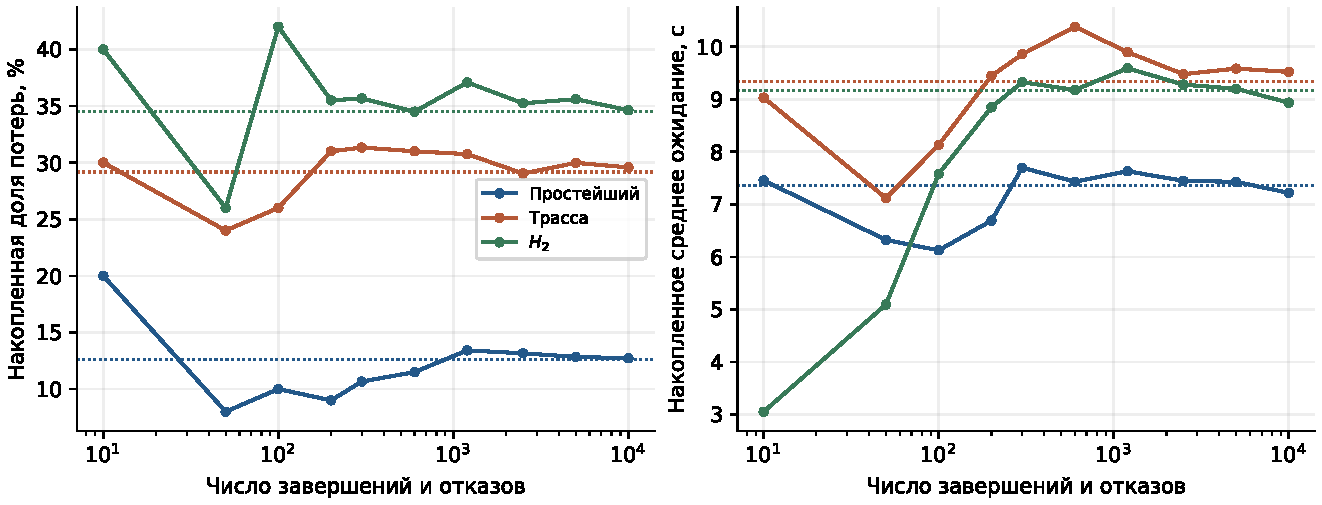
\includegraphics[width=.93\textwidth]{../out/part1/gpss/transition.pdf}
 \caption{Переход из пустого состояния при \(\rho_1=0{,}75\).
 Пунктиром показаны средние после прогрева}
 \label{fig:p1-transition}
\end{figure}

\subsection{Ёмкость накопителей и число приборов}

При простейшем входе и экспоненциальном обслуживании обеим ветвям
выделяли одинаковое число мест ожидания. Таблица~\ref{tab:p1-buffers}
показывает исходные режимы, результаты с восьмью местами на ветвь
и первые из проверенных ёмкостей, при которых во всех повторах
отсутствовали отказы за измерительный интервал, вместе с ближайшими
меньшими ёмкостями на сетке. По
рисунку~\ref{fig:p1-buffers} виден обмен между длиной ожидания и
долей потерь. При \(\rho_1=0{,}90\) восемь мест ожидания на ветвь
снизили потери с \(41{,}20\%\) до \(4{,}49\%\), при этом среднее
ожидание выросло с нуля до \(35{,}00\) с. Первые из проверенных
ёмкостей без отказов составили \(32\) и \(128\) мест на ветвь при
\(\rho_1=0{,}50\) и \(0{,}90\) соответственно. При \(256\) местах
максимальные длины очереди среди ветвей и повторов равны \(18\) и
\(99\). Оценка достаточной ёмкости зависит от длительности
наблюдения и генераторов. При
неограниченной длительности обслуживания и положительной
интенсивности потока любой конечный накопитель может переполниться.

\begin{table}[htbp]
 \centering\small
 \caption{Потери и времена при выбранных ёмкостях накопителей}
 \label{tab:p1-buffers}
 \begin{tabular}{@{}rrrrrr@{}}
 \toprule
 \(\rho_1\) & Мест на ветвь & Отказов & Потери, \% &
 \(\overline W\), с & \(\overline T\), с\\
 \midrule
 \TableRows ../out/part1/gpss/buffers_rows.tex
 \bottomrule
 \end{tabular}
\end{table}

\begin{figure}[htbp]
 \centering
 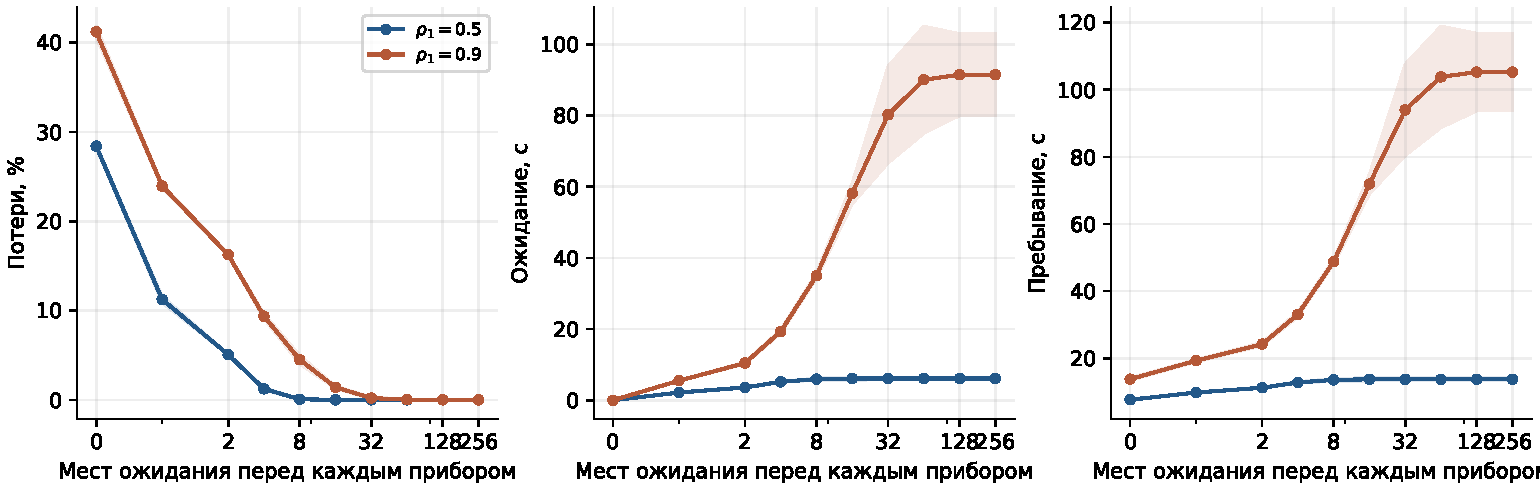
\includegraphics[width=\textwidth]{../out/part1/gpss/buffers.pdf}
 \caption{Потери и задержки при изменении ёмкости накопителей}
 \label{fig:p1-buffers}
\end{figure}

Для одного прибора весь поток направляется в одну очередь с двумя
местами ожидания. Исходная схема с двумя приборами сохраняет
разветвление \(0{,}75/0{,}25\). Третий прибор добавляется в первую
ветвь и обслуживает её общую очередь. При сравнении сохраняется
интенсивность входа, а среднее время обслуживания либо оставляется
тем же, либо подбирается под одинаковую предложенную загрузку
одного прибора первой ветви. Если в первой ветви \(c_1\) приборов
и вероятность выбора этой ветви равна \(p_1\), загрузка рассчитывается
как \(p_1 b/(c_1 a)\).

\begin{table}[htbp]
 \centering\small
 \caption{Число приборов при исходной загрузке \(\rho_1=0{,}75\)}
 \label{tab:p1-servers}
 \begin{tabular}{@{}lrrrrr@{}}
 \toprule
 Фиксируется & Приборов & \(\rho_1\) & \(b\), с &
 \(\overline W\), с & \(\overline T\), с\\
 \midrule
 \TableRows ../out/part1/gpss/servers_rows.tex
 \bottomrule
 \end{tabular}
\end{table}

При одинаковом времени обслуживания увеличение числа приборов
с одного до трёх снизило среднее ожидание с \(11{,}43\) до \(1{,}55\) с,
а среднее пребывание — с \(22{,}89\) до \(13{,}03\) с. В серии
с одинаковой загрузкой пребывание при трёх приборах выросло до
\(30{,}30\) с. Время обслуживания в этом опыте увеличивалось
вместе с числом приборов и непосредственно входило во время пребывания.

\begin{figure}[htbp]
 \centering
 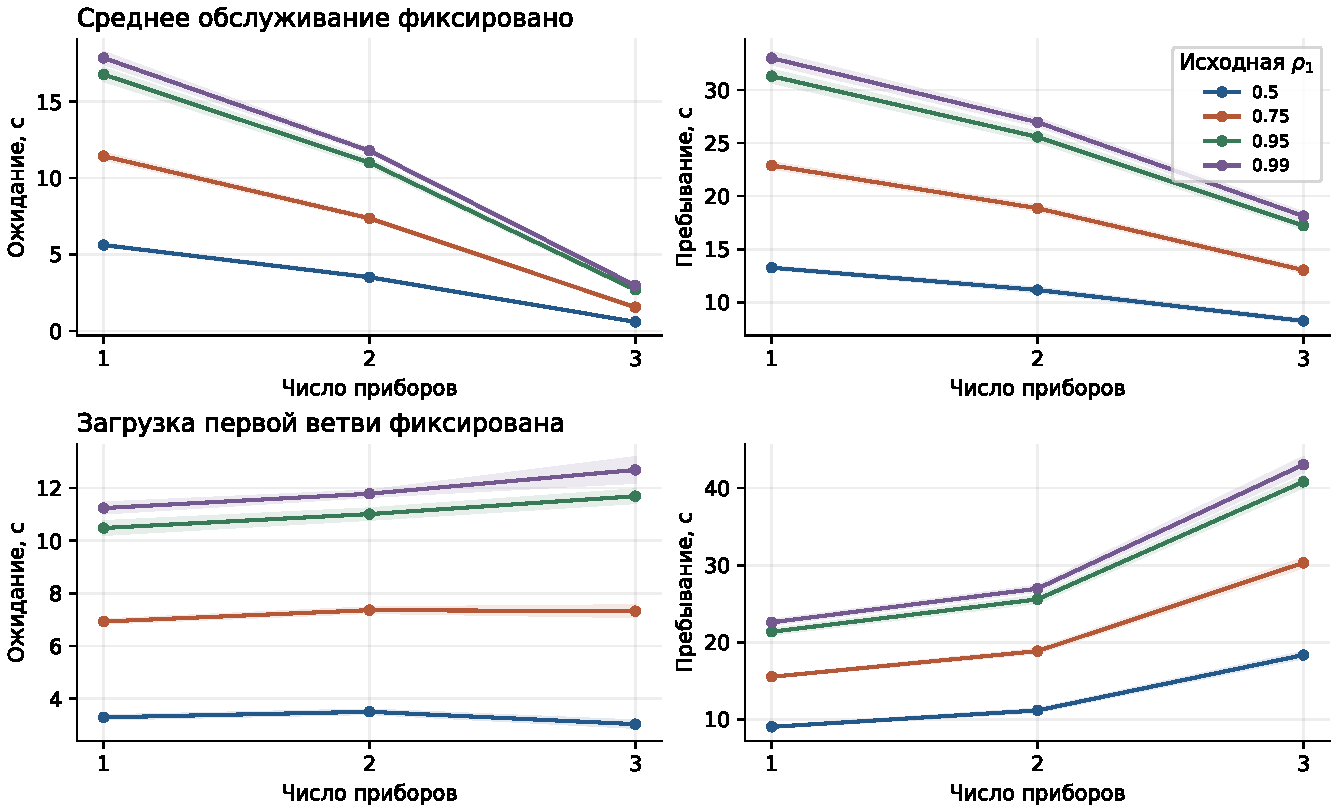
\includegraphics[width=.92\textwidth]{../out/part1/gpss/servers.pdf}
 \caption{Влияние числа приборов. В верхнем ряду фиксировано
 среднее обслуживание, в нижнем — загрузка первой ветви}
 \label{fig:p1-servers}
\end{figure}

\subsection{Проверка по формулам и форма распределений}

В контрольных прогонах использовалась одноканальная СМО с
простейшим потоком и накопителем на \(256\) мест. Для среднего
ожидания и пребывания при \(\rho=\lambda b<1\) использована
формула Поллачека — Хинчина
\[
 \overline W=\frac{\lambda\,\mathrm E[S^2]}{2(1-\rho)}
             =\frac{\rho b(1+c_s^2)}{2(1-\rho)},\qquad
 \overline T=\overline W+b.
\]
Здесь \(S\) — время обслуживания, \(c_s\) — его коэффициент
вариации. Для \(M/M/1\) принято \(c_s=1\), для \(M/G/1\) с
\(H_2\)-обслуживанием \(c_s=2\). В таблице~\ref{tab:p1-controls}
относительное отклонение \(\Delta_W\) рассчитано от теоретического
ожидания. В четырёх контрольных режимах потерь не наблюдалось.
Расхождение среднего ожидания с аналитическим расчётом не превысило
\(1{,}64\%\) для \(M/M/1\) и \(1{,}45\%\) для \(M/G/1\).

\begin{table}[htbp]
 \centering\small
 \caption{Сравнение одноканальных контролей с аналитическим расчётом}
 \label{tab:p1-controls}
 \begin{tabular}{@{}lrrrrrrr@{}}
 \toprule
 Модель & \(\rho\) &
 \(W_\text{расч}\), с & \(W_\text{GPSS}\), с & \(\Delta_W\), \% &
 \(T_\text{расч}\), с & \(T_\text{GPSS}\), с & Отказов\\
 \midrule
 \TableRows ../out/part1/gpss/controls_rows.tex
 \bottomrule
 \end{tabular}
\end{table}

\begin{table}[htbp]
 \centering\small
 \caption{Коэффициенты вариации задержек при \(\rho_1=0{,}75\)}
 \label{tab:p1-variation}
 \begin{tabular}{@{}lrrrr@{}}
 \toprule
 Поток & \(P(W=0)\), \% & \(c_W\) & \(c_{W\mid W>0}\) & \(c_T\)\\
 \midrule
 \TableRows ../out/part1/gpss/variation_rows.tex
 \bottomrule
 \end{tabular}
\end{table}

Ожидание имеет массу в нуле и положительную составляющую. Для
положительных задержек коэффициент вариации в четырёх опытах
лежит в пределах \(0{,}90\)–\(0{,}92\), а для пребывания —
\(0{,}86\)–\(0{,}92\). По относительному разбросу эти величины
близки к экспоненциальным. Для идентификации закона нужны данные
о форме распределения, в частности частоты из таблиц GPSS World.
